\documentclass[xcolor={cmyk}]{beamer}
\usepackage[utf8]{inputenc}
\usepackage[T1]{fontenc}
\usepackage[english]{babel}
\usepackage{verbatim}
\graphicspath{{./pics/}}

\title{4G LTE CoMP, Coordinated Multipoint}
\subtitle{4th Semester Institute Project}
\author[Matthis Dirksen]{\tiny Leonhard Hetz \and Philipp Braun \and Carmine Bianco \and Alissa Wenzel \and Matthis Dirksen}
\date{July 21, 2016}

% Select theme
\usetheme[english]{RWTH_Ti}
\setbeamercolor*{block body}{bg = white}

\begin{document}

% Titlepage
\frame[plain]{\titlepage}

% Template for the slides: 
\begin{comment}
 
 \begin{frame}{4G LTE CoMP, Coordinated Multipoint}{4th Semester Institute Project}
	 \begin{block}{...}
	
	 \end{block}
 \end{frame}
 
 \end{comment}

% Content Slide
\begin{frame}{4G LTE CoMP, Coordinated Multipoint}{4th Semester Institute Project}
	\begin{block}{Content}
		\begin{columns}
			\begin{column}{.9\textwidth}
				\begin{itemize}
					\item Introduction
					\item Background
					\item System Model
					\item Simulation
					\item Evaluations
					\item Conclusions
					\item References
				\end{itemize}
			\end{column}
		\end{columns}
	\end{block}
\end{frame}

% Content Slide highlight Motivation 
\begin{frame}{4G LTE CoMP, Coordinated Multipoint}{4th Semester Institute Project}
	\begin{block}{Content}
		\begin{columns}
			\begin{column}{.9\textwidth}
				\begin{itemize}
					\item \textbf{\emph{Introduction}}
					\begin{itemize}
						\item \textbf{\emph{Motivation}}
					\end{itemize}
					\item Background
					\item System Model
					\item Simulation
					\item Evaluations
					\item Conclusions
					\item References
				\end{itemize}
			\end{column}
		\end{columns}
	\end{block}
\end{frame}

% Motivation Slide
 \begin{frame}{4G LTE CoMP, Coordinated Multipoint}{4th Semester Institute Project}
	 \begin{block}{Motivation}
	 	\begin{columns}
			\begin{column}{.9\textwidth}
				\begin{itemize}
					\item CoMP: optimizing performance by sending and receiving data to and from User Entities from several points
					\item Especially important on cell edges
					\item Aim: improving quality for user, optimum capacity of network 
					\item CoMP still in development (not included in LTE Rel. 10)
				\end{itemize}
			\end{column}
		\end{columns}
	 \end{block}
 \end{frame}
 
 % Content Slide highlight Background 
\begin{frame}{4G LTE CoMP, Coordinated Multipoint}{4th Semester Institute Project}
	\begin{block}{Content}
		\begin{columns}
			\begin{column}{.9\textwidth}
				\begin{itemize}
					\item Introduction
					\item \textbf{\emph{Background}}
					\item System Model
					\item Simulation
					\item Evaluations
					\item Conclusions
					\item References
				\end{itemize}
			\end{column}
		\end{columns}
	\end{block}
\end{frame}

% BACKGROUND SLIDES

% General information of research
 \begin{frame}{Background - Overview on research}
	 \begin{block}{Background}
	 	\begin{columns}
			\begin{column}{.9\textwidth}
				\begin{itemize}
					\item Papers on LTE-A, Joint Transmission, Beamforming and CoMP in general
					\item Reference: MATLAB-based down-
link physical-layer simulator for LTE (Mehlführer, C., 2009)
					\begin{itemize}
						\item MATLAB-based downlink physical-layer simulator for LTE
						\item covering Multi-Cell Multi-User simulation scenarios -> most realistic
					\end{itemize}
				\end{itemize}
			\end{column}
		\end{columns}
	 \end{block}
 \end{frame}
 
 % CoMP - overview
 \begin{frame}{Background - overview on CoMP}
 	\begin{block}{CoMP - overview}
		\begin{columns}
			\begin{column}{.9\textwidth}
				\begin{itemize}
					\item LTE Advanced:
					\item CoMP: Coordinate MultiPoint operation
					\begin{itemize}
						\item refers to wide range of techniques
						\item dynamic coordination or transmission and reception with multiple geographically separated eNBs (base stations)
						\item goal: enhancing overall system performance, more effective use of resources, improved end user service quality (especially at the cell edges)
					\end{itemize}
				\end{itemize}
			\end{column}
		\end{columns}
	 \end{block}
 \end{frame}
 
% CoMP - Major Categories
 \begin{frame}{Background - CoMP: major categories}
 	\begin{block}{CoMP: major categories}
		\begin{columns}
			\column{.5\textwidth}
				Coordinated Scheduling (CS) / Coordinated Beamforming (CB)
			\column{.5\textwidth}
			Joint Processing (JP)
				\begin{itemize}
					\item Joint Transmission (JT)
					\item Dynamic Point Selection (DPS)
					\begin{itemize}
						\item with muting
						\item without muting
					\end{itemize}
				\end{itemize}
		\end{columns}
	 \end{block}
 \end{frame}
 
 % Coordinated Scheduling
 \begin{frame}{Background - Coordinated Scheduling}
 	\begin{block}{Coordinated Scheduling (CS)}
		\begin{columns}
			\begin{column}{.9\textwidth}
				\begin{itemize}
					\item data available at one node
					\item transfered packets do not overlap in time
					\item TODO insert graphic: timesteps
				\end{itemize}
			\end{column}
		\end{columns}
	 \end{block}
 \end{frame}

% Dynamic Point Selection
 \begin{frame}{Background - Dynamic Point Selection}
 	\begin{block}{Dynamic Point Selection (DPS)}
		\begin{columns}
			\begin{column}{.9\textwidth}
				\begin{itemize}
					\item data usually available at several nodes
					\item user decides per packet which base station is best
					\item TODO insert graphic: timesteps
				\end{itemize}
			\end{column}
		\end{columns}
	 \end{block}
 \end{frame}
 
 % Scheduling
 \begin{frame}{Background - Scheduling}
 	\begin{block}{Coordinated Scheduling}
		\begin{columns}
			\begin{column}{.9\textwidth}
				\begin{itemize}
					\item assignment of resource blocks (RB) to each user
					\item i.e. Round Robin (timeslots divided equally between users)
					\item dynamic scheduling: mapping RBs to users based on different criteria
				\end{itemize}
			\end{column}
		\end{columns}
	 \end{block}
 \end{frame}

% SINR
 \begin{frame}{Background - SINR}
 	\begin{block}{SINR}
		\begin{columns}
			\begin{column}{.9\textwidth}
				\begin{itemize}
					\item signal-to-interference-plus-noise ratio
					\begin{equation}
\frac{S}{I + N}
					\end{equation}
					\begin{itemize}
						\item S = power of signal
						\item I = power of interference
						\item N = power of noise
					\end{itemize}
					\item used to determine signal quality
				\end{itemize}
			\end{column}
		\end{columns}
	 \end{block}
 \end{frame}

% CQI and channel modulation
 \begin{frame}{Background - CQI and channel modulation}
 	\begin{block}{CQI and channel modulation}
		\begin{columns}
			\begin{column}{.9\textwidth}
				\begin{itemize}
					\item Channel Quality Indicator
					\item determines modulation
					\begin{itemize}
						\item transfer block size (TBS)
						\item resource blocks for users
					\end{itemize}
					\item depends on SINR
					\item Best CQI scheduling: maximation of rate, but unfair (only UEs with very good channels get scheduled at all) -> "fair" modulation necessary
				\end{itemize}
			\end{column}
		\end{columns}
	 \end{block}
 \end{frame}

 % Content Slide highlight System Model 
\begin{frame}{4G LTE CoMP, Coordinated Multipoint}{4th Semester Institute Project}
	\begin{block}{Content}
		\begin{columns}
			\begin{column}{.9\textwidth}
				\begin{itemize}
					\item Introduction
					\item Background
					\item \textbf{\emph{System Model}}
					\item Simulation
					\item Evaluations
					\item Conclusions
					\item References
				\end{itemize}
			\end{column}
		\end{columns}
	\end{block}
\end{frame}

% System Model Slide
 \begin{frame}{4G LTE CoMP, Coordinated Multipoint}{4th Semester Institute Project}
	 \begin{block}{System Model - Assumptions}
	 	\begin{columns}
			\begin{column}{.9\textwidth}
				\begin{itemize}
					\item it is always known where a UE is 
					\item UE does not move so no Dopplereffect or similar effects
					\item CQI, PMI, RI are randomly generated
					\item fixed number of UEs in a simulation
					\item using mean value of the Rayleigh distribution (provided from 3GPP)
					\item basestations are always in a hexagonal layout
				\end{itemize}
			\end{column}
		\end{columns}
	 \end{block}
 \end{frame}
 
% System Model Slide
 \begin{frame}{4G LTE CoMP, Coordinated Multipoint}{4th Semester Institute Project}
	 \begin{block}{System Model - Programming}
	 	\begin{columns}
			\begin{column}{.9\textwidth}
				\begin{itemize}
					\item Classes providing main functionality: central unit, base station, user entity, channel
					\item Classes providing background data and auxiliary functions: TBS, helpers, params, precoding matrix
				\end{itemize}
			\end{column}
		\end{columns}
	 \end{block}
 \end{frame}
 
 
 % Details on our Classes
  \begin{frame}{4G LTE CoMP, Coordinated Multipoint}{4th Semester Institute Project}
	 \begin{block}{System Model - Classes providing main functionality}
	 	\begin{columns}
			\begin{column}{.9\textwidth}
				\begin{itemize}
					\item Central Unit: coordinates all base stations 
						\begin{itemize}
							\item one CU per simulation
						\end{itemize}
					\item Base Station: matches subcarriers to connected users, calculates modulation
					\item User Entity: returns feedback to the base station
					\item Channel: has a certain frequency and amount of subcarriers
					\begin{itemize}
						\item Friis equation for calculation of path loss
						\item model: Rayleigh channel
					\end{itemize}
				\end{itemize}
			\end{column}
		\end{columns}
	 \end{block}
 \end{frame}
 
 % Slide with overview of the classes
  \begin{frame}{4G LTE CoMP, Coordinated Multipoint}{4th Semester Institute Project}
	 \begin{block}{Overview of the classes}
		 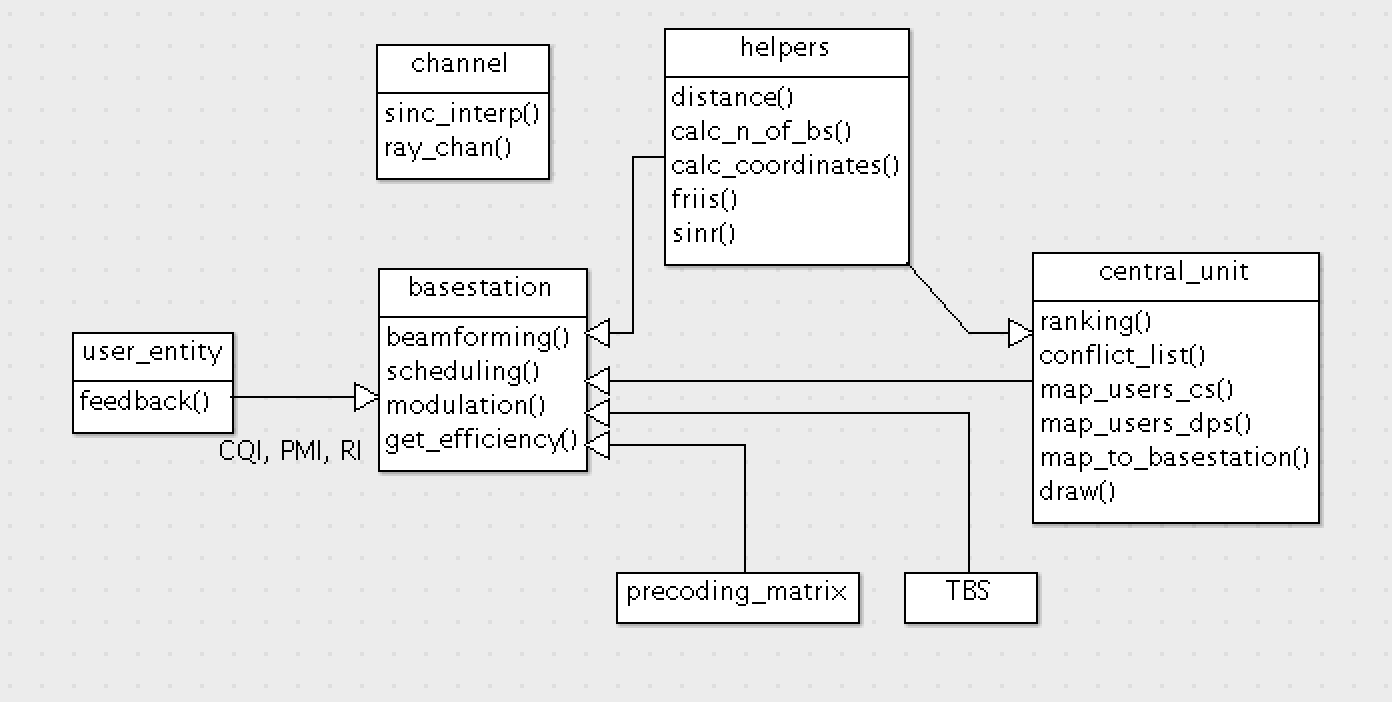
\includegraphics[width=\linewidth,height=\textheight,keepaspectratio]{klassen.png}
	 \end{block}
 \end{frame}

 % Content Slide highlight Simulation
\begin{frame}{4G LTE CoMP, Coordinated Multipoint}{4th Semester Institute Project}
	\begin{block}{Content}
		\begin{columns}
			\begin{column}{.9\textwidth}
				\begin{itemize}
					\item Introduction
					\item Background
					\item System Model
					\item \textbf{\emph{Simulation}}
					\item Evaluations
					\item Conclusions
					\item References
				\end{itemize}
			\end{column}
		\end{columns}
	\end{block}
\end{frame}

% Simulation Slide
% What is it able to do?
 \begin{frame}{4G LTE CoMP, Coordinated Multipoint}{4th Semester Institute Project}
	 \begin{block}{Simulation - main characteristics}
	 	\begin{columns}
			\begin{column}{.9\textwidth}
				\begin{itemize}
					\item Flexibility
					\item Simulation Process
					\begin{itemize}
						\item Initialization
						\item Simulation Cycle
						\begin{itemize}
							\item mapping of users to basestations
							\item assignment of recourceblocks to users
							\item calculation of the best modulation and coding scheme
					 	\end{itemize}
					 \end{itemize}
					
				 \end{itemize}
			\end{column}
		\end{columns}
	 \end{block}
 \end{frame}
 
% simulation slide II
 \begin{frame}{4G LTE CoMP, Coordinated Multipoint}{4th Semester Institute Project}
 \begin{block}{Simulation DPS I}
 
 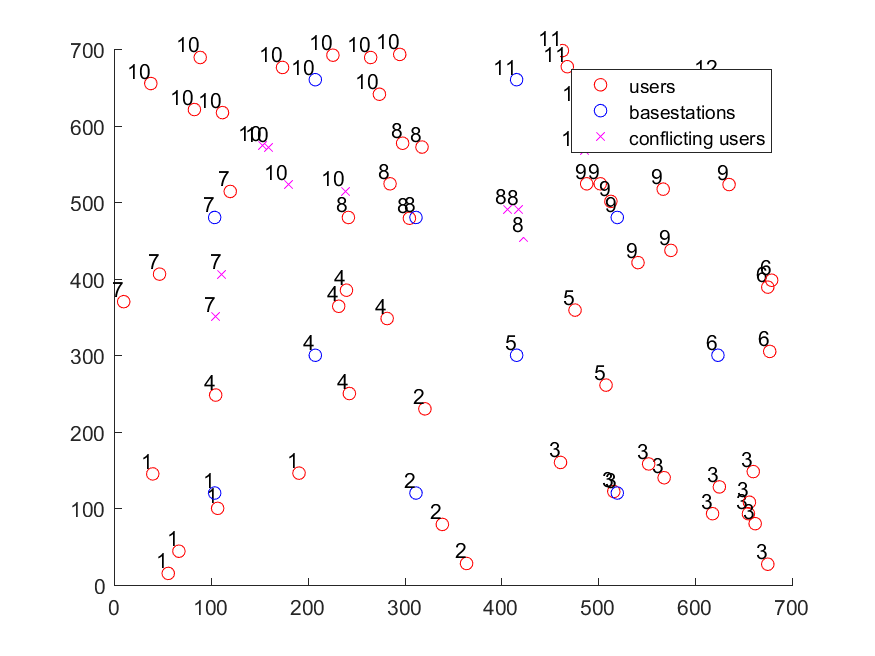
\includegraphics[width=\linewidth,height=\textheight,keepaspectratio]{MapPlotDPS1.png}
 \end{block}
 \end{frame}
 
 % simulation slide III
 \begin{frame}{4G LTE CoMP, Coordinated Multipoint}{4th Semester Institute Project}
 \begin{block}{Simulation DPS II}
 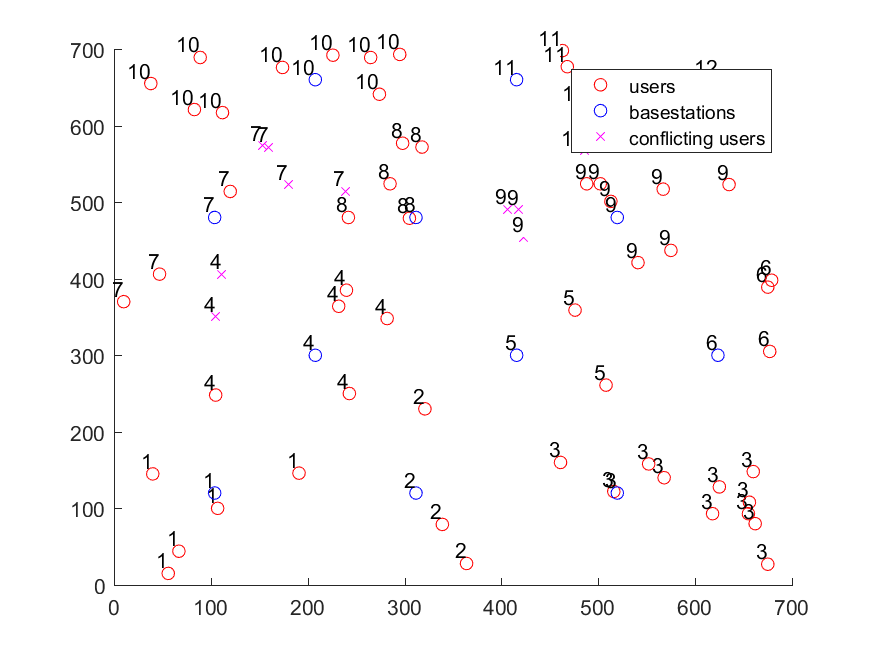
\includegraphics[width=\linewidth,height=\textheight,keepaspectratio]{MapPlotDPS2.png}
 \end{block}
 \end{frame}
 
 % simulation slide II
 \begin{frame}{4G LTE CoMP, Coordinated Multipoint}{4th Semester Institute Project}
 \begin{block}{Simulation CS I}
 
 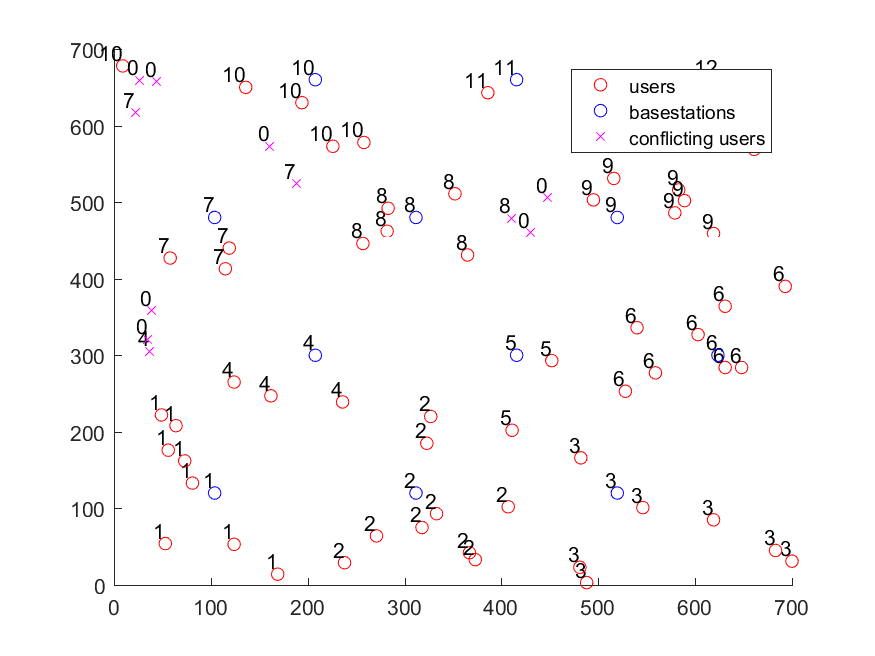
\includegraphics[width=\linewidth,height=\textheight,keepaspectratio]{MapPlotCS1.png}
 \end{block}
 \end{frame}
 
 % simulation slide III
 \begin{frame}{4G LTE CoMP, Coordinated Multipoint}{4th Semester Institute Project}
 \begin{block}{Simulation CS II}
 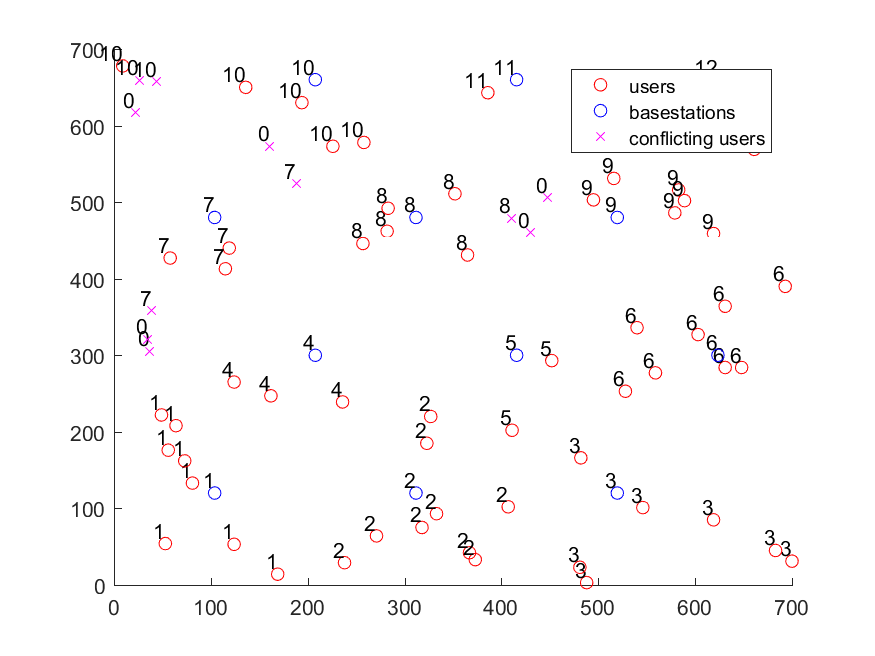
\includegraphics[width=\linewidth,height=\textheight,keepaspectratio]{MapPlotCS2.png}
 \end{block}
 \end{frame}
 
 % Content Slide highlight Evaluation
\begin{frame}{4G LTE CoMP, Coordinated Multipoint}{4th Semester Institute Project}
	\begin{block}{Content}
		\begin{columns}
			\begin{column}{.9\textwidth}
				\begin{itemize}
					\item Introduction
					\item Background
					\item System Model
					\item Simulation
					\item \textbf{\emph{Evaluation}}
					\item Conclusions
					\item References
				\end{itemize}
			\end{column}
		\end{columns}
	\end{block}
\end{frame}
 
% Evaluations Slide
% Simulation with and without Comp
% why should you use CoMP
 \begin{frame}{4G LTE CoMP, Coordinated Multipoint}{4th Semester Institute Project}
	 \begin{block}{Evaluation}
	 	\begin{columns}
			\begin{column}{.9\textwidth}
				\begin{itemize}
					\item Cost = additional backhaul
					\item Use = less interference at cell edges
					\item (I need graphics for the following slides)
				\end{itemize}
			\end{column}
		\end{columns}
	 \end{block}
 \end{frame}
 
 % Slide on why to use CoMP
 \begin{frame}{4G LTE CoMP, Coordinated Multipoint}{4th Semester Institute Project}
	 \begin{block}{Advantages}
	 	\begin{columns}
			\begin{column}{.9\textwidth}
				\begin{itemize}
					\item CoMP allows better allocation for users at cell edges --> more receiving power
					\item Utilization of different subcarriers inside conflict zones avoids interference
				\end{itemize}
			\end{column}
		\end{columns}
	 \end{block}
	 \begin{block}{Disadvantages}
	 	\begin{columns}
			\begin{column}{.9\textwidth}
				\begin{itemize}
					\item Computational power and time loss
					\item Bigger signaling overhead between users and base stations
					\item More frequent communication with the CU --> bigger backhaul needed
				\end{itemize}
			\end{column}
		\end{columns}
	 \end{block}
 \end{frame}

 
  % Content Slide highlight Conclusions
\begin{frame}{4G LTE CoMP, Coordinated Multipoint}{4th Semester Institute Project}
	\begin{block}{Content}
		\begin{columns}
			\begin{column}{.9\textwidth}
				\begin{itemize}
					\item Introduction
					\item Background
					\item System Model
					\item Simulation
					\item Evaluations
					\item \textbf{\emph{Conclusions}}
					\item References
				\end{itemize}
			\end{column}
		\end{columns}
	\end{block}
\end{frame}

% Conclusions Slide
\begin{frame}{4G LTE CoMP, Coordinated Multipoint}{4th Semester Institute Project}
	\begin{block}{Conclusion}
		\begin{columns}
			\begin{column}{.9\textwidth}
				\begin{itemize}
					\item Main functionalities for a LTE-Advanced simulator implemented
					\begin{itemize}
						\item Implementation of \textbf{Coordinated Scheduling} and \textbf{Dynamic Point Selection}
						\item Comparison with system behaviour without CoMP
					\end{itemize}
					\item Advantages of CoMP mainly for users at cell edges
					\begin{itemize}
						\item Profitability vs backhaul/signaling trade-offs should be evaluated on a case-by-case basis
						\item Possible solution: activating Coordinated Multipoint only as a certain conflict density in the simulated environment is reached
					\end{itemize}
				\end{itemize}
			\end{column}
		\end{columns}
	\end{block}
\end{frame}

%Conclusions #2: which (factual) goals did we reach in the project?
\begin{frame}{4G LTE CoMP, Coordinated Multipoint}{4th Semester Institute Project}
	 \begin{block}{Project goals reached}
	 	\begin{columns}
			\begin{column}{.9\textwidth}
				\begin{itemize}
					\item Analysis of behaviour of frequency flat, slow fading channels
					\item Differences between SISO and MIMO channel models and their implications
					\item Criteria for estabishling a state of conflict between different user entities
					\item Choice of channel modulation based upon generated feedback
					\item Allocating users to base stations according to selected CoMP scheme
				\end{itemize}
			\end{column}
		\end{columns}
	 \end{block}
 \end{frame}

%Conclusions #3: what did we learn (soft skills et al.) by working on this project (on two slides)

\begin{frame}{4G LTE CoMP, Coordinated Multipoint}{4th Semester Institute Project}
	 \begin{block}{Learning goals reached}
	 	 \hspace*{.1\linewidth}\begin{minipage}{.8\linewidth}
    		\begin{block}{Programming}
      			\begin{itemize}
      				\item \textbf{Object-oriented programming} on MATLAB
      				\item Graphical representation of simulation results
      				\item Working with parameter files/external files (e.g. precoding matrix) and already existing MATLAB libraries
      				\item Defining model simplifications while still mantaining a degree of correctness
      			\end{itemize}
    		\end{block}
    	\end{minipage}
	 \end{block}	 
 \end{frame}

\begin{frame}{4G LTE CoMP, Coordinated Multipoint}{4th Semester Institute Project}
	 \begin{block}{Learning goals reached}
    	\hspace*{.1\linewidth}\begin{minipage}{.8\linewidth}
    		\begin{block}{Soft skills}
      			\begin{itemize}
      				\item Collection of preliminary informations through approach to English language scientific literature
      				\item Teamwork: weekly meetings and frequent contacts with the project supervisors
      				\begin{itemize}
      					\item Task division in the team according to current needs and time availability
      				\end{itemize}
      				\item Debugging and version control on GitHub
      				\item \LaTeX basics for the final presentation
      			\end{itemize}
    		\end{block}
    	\end{minipage}
	 \end{block}	 
 \end{frame}

%Last slide: possible expansions: what could still be done?
 \begin{frame}{4G LTE CoMP, Coordinated Multipoint}{4th Semester Institute Project}
	 \begin{block}{What comes next?}
	 	\begin{columns}
			\begin{column}{.9\textwidth}
				\begin{itemize}
					\item Implementation of other CoMP schemes, e.g. coordinated beamforming
					\item Different channel models (e.g. \textit{fast fading} channels)
					\item Further optimization of CU/BS
					\begin{itemize}
						\item Different allocation of implementation stages between CU and BS
						\item More refined scheduling patterns (currently implemented: Round Robin)
					\end{itemize}
					\item Implementation of different environment setups and parameters
				\end{itemize}
			\end{column}
		\end{columns}
	 \end{block}
 \end{frame}


  % Content Slide highlight References
\begin{frame}{4G LTE CoMP, Coordinated Multipoint}{4th Semester Institute Project}
	\begin{block}{Content}
		\begin{columns}
			\begin{column}{.9\textwidth}
				\begin{itemize}
					\item Introduction
					\item Background
					\item System Model
					\item Simulation
					\item Evaluations
					\item Conclusions
					\item \textbf{\emph{References}}
				\end{itemize}
			\end{column}
		\end{columns}
	\end{block}
\end{frame}

% References Slide
% Papers etc.
 \begin{frame}{4G LTE CoMP, Coordinated Multipoint}{4th Semester Institute Project}
	 \begin{block}{References}
	 	\begin{columns}
			\begin{column}{.9\textwidth}
				\begin{itemize}
					\item Mehlführer, C. et al, 2009. Simulating The Long Term Evolution Physical Layer. Proc. 17th European Signal Processing Conference (EUSIPCO 2009), [online]
					\item Davydov, A. et al, 2013. Evaluation of Joint Transmission CoMP in C-RAN based LTE-A HetNets with Large Coordination Areas. Globecom 2013 Workshop.
					\item Hong, M. et al, 2012. Joint Base Station Clustering and Beamformer Design for Partial Coordinated Transmission in Heterogeneous Networks.
					\item Sawahashi, M. et al, 2010. Coordinated Multipoint Transmission/Reception Techniques For LTE-Advanced.
				\end{itemize}
			\end{column}
		\end{columns}
	 \end{block}
 \end{frame}
 
 % Last Slide
  \begin{frame}{4G LTE CoMP, Coordinated Multipoint}{4th Semester Institute Project}
	\begin{block}{Thank you for your attention!}
	\end{block}
 \end{frame}


\end{document}